\documentclass[11pt,]{article}
\usepackage{lmodern}
\usepackage{amssymb,amsmath}
\usepackage{ifxetex,ifluatex}
\usepackage{fixltx2e} % provides \textsubscript
\ifnum 0\ifxetex 1\fi\ifluatex 1\fi=0 % if pdftex
  \usepackage[T1]{fontenc}
  \usepackage[utf8]{inputenc}
\else % if luatex or xelatex
  \ifxetex
    \usepackage{mathspec}
  \else
    \usepackage{fontspec}
  \fi
  \defaultfontfeatures{Ligatures=TeX,Scale=MatchLowercase}
\fi
% use upquote if available, for straight quotes in verbatim environments
\IfFileExists{upquote.sty}{\usepackage{upquote}}{}
% use microtype if available
\IfFileExists{microtype.sty}{%
\usepackage{microtype}
\UseMicrotypeSet[protrusion]{basicmath} % disable protrusion for tt fonts
}{}
\usepackage[margin=1in]{geometry}
\usepackage{hyperref}
\hypersetup{unicode=true,
            pdfborder={0 0 0},
            breaklinks=true}
\urlstyle{same}  % don't use monospace font for urls
\usepackage{graphicx,grffile}
\makeatletter
\def\maxwidth{\ifdim\Gin@nat@width>\linewidth\linewidth\else\Gin@nat@width\fi}
\def\maxheight{\ifdim\Gin@nat@height>\textheight\textheight\else\Gin@nat@height\fi}
\makeatother
% Scale images if necessary, so that they will not overflow the page
% margins by default, and it is still possible to overwrite the defaults
% using explicit options in \includegraphics[width, height, ...]{}
\setkeys{Gin}{width=\maxwidth,height=\maxheight,keepaspectratio}
\IfFileExists{parskip.sty}{%
\usepackage{parskip}
}{% else
\setlength{\parindent}{0pt}
\setlength{\parskip}{6pt plus 2pt minus 1pt}
}
\setlength{\emergencystretch}{3em}  % prevent overfull lines
\providecommand{\tightlist}{%
  \setlength{\itemsep}{0pt}\setlength{\parskip}{0pt}}
\setcounter{secnumdepth}{5}
% Redefines (sub)paragraphs to behave more like sections
\ifx\paragraph\undefined\else
\let\oldparagraph\paragraph
\renewcommand{\paragraph}[1]{\oldparagraph{#1}\mbox{}}
\fi
\ifx\subparagraph\undefined\else
\let\oldsubparagraph\subparagraph
\renewcommand{\subparagraph}[1]{\oldsubparagraph{#1}\mbox{}}
\fi

%%% Use protect on footnotes to avoid problems with footnotes in titles
\let\rmarkdownfootnote\footnote%
\def\footnote{\protect\rmarkdownfootnote}

%%% Change title format to be more compact
\usepackage{titling}

% Create subtitle command for use in maketitle
\newcommand{\subtitle}[1]{
  \posttitle{
    \begin{center}\large#1\end{center}
    }
}

\setlength{\droptitle}{-2em}
  \title{}
  \pretitle{\vspace{\droptitle}}
  \posttitle{}
  \author{}
  \preauthor{}\postauthor{}
  \date{}
  \predate{}\postdate{}


\begin{document}

\begin{center}
\Large\scshape{Business Confidence and the Business Cycle in South Africa} \\ 
\vspace{1em}
\large\normalfont{Laurie H. Binge}\footnote{PhD candidate at the Department of Economics at Stellenbosch University. Corresponding author email address: lhbinge@gmail.com},
\large\normalfont{Willem H. Boshoff}\footnote{Associate Professor at the Department of Economics at Stellenbosch University. Email address: wimpie2@sun.ac.za} \\
\normalsize\textit{Stellenbosch University, Stellenbosch, South Africa.} \\
\normalsize\normalfont{\today} 
\end{center}\begin{small}

Business confidence indicators are widely used leading indicators of economic activity. The potential role of low confidence and heightened uncertainty in shaping economic outcomes has also motivated a large international literature investigating the impact of changes in business sentiment on real economic activity. It is therefore important to measure business confidence as accurately as possible. This chapter constructs improved composite indicators of business confidence for South Africa, based on the microdata from the BER's business tendency surveys. The new confidence indicators are used to examine whether there is a significant positive relationship between confidence and real GDP growth, the timing of this relationship, and whether it remains significant after taking other economic variables into account. The composite confidence indicators improve on existing indicators in that they exhibit higher correlation with real GDP growth and higher concordance with the official SARB business cycle. The new indicators contain useful information about current and future economic developments. 

\vspace{0.5em}
\noindent{\textbf{JEL Classification:} C83, D81, E32} \\
    \noindent{\textbf{Keywords:} Business Tendency Surveys, Confidence, Business Cycle Indicators}
\end{small}\renewcommand{\thefootnote}{\arabic{footnote}}

\renewcommand{\thefootnote}{\arabic{footnote}}

\section{Introduction}\label{introduction}

Business confidence indicators, such as the European Commission's
Economic Sentiment Index, are popular and useful leading indicators of
economic activity in many countries (United Nations, 2015). This is also
the case in South Africa, where the Bureau for Economic Research's
Business Confidence Index (BER BCI) is often quoted in the media and is
used by the SARB as a leading indicator to identify official business
cycle turning points (Bosch, 2015). Given that business confidence
indicators are popular and potentially useful, it is important to
measure them as accurately as possible.

Only two business confidence indicators are regularly published for
South Africa: the BER BCI and the South African Chamber of Commerce and
Industry Business Confidence Index (SACCI BCI). Both have some
shortcomings. The SACCI BCI is a composite measure of economic activity,
rather than a measure of confidence in the way it is defined in the
literature. The BER BCI is a measure of confidence derived from the
BER's business tendency surveys. It is based on a single question,
weighted in an ad hoc manner, and excludes the services sector
altogether.

This chapter estimates new proxies for business confidence in South
Africa using micro-data from the BER business tendency surveys, with the
aim of improving on the existing measures. Although measuring business
confidence is challenging, survey-based indicators can be helpful in
discovering key economic agents' opinions on current and future economic
developments (Girardi and Reuter, 2017). Survey-based confidence
indicators have the advantage that they are published long before the
official statistics become available and are not subject to revision
(European Central Bank, 2013).

The idea that weak business confidence and heightened uncertainty
contributed to a large extent to the Great Recession and to the
lacklustre subsequent recovery has inspired a substantial international
literature examining the impact of changes in sentiment on output and
investment decisions. The International Monetary Fund (2017) cited
elevated political uncertainty and weak consumer and business confidence
when it marked down South Africa's growth forecast for 2018. Yet, to
date there has been little research on business confidence in South
Africa (e.g. Pellissier (2002)), in part due to the difficulty of
measurement.

This chapter investigates the relationship between the survey-based
business confidence indicators and real economic activity in South
Africa. The aim is to study whether there is a significant positive
relationship between the indicators and real GDP growth, the timing of
this relationship, and whether it remains significant after taking other
economic variables into account.

\section{Confidence}\label{confidence}

Business confidence involves firms' perceptions of, or degree of
optimism regarding, current business conditions and the expected future
business climate (Mendicino and Punzi, 2013). In this chapter, firms'
perceptions of current and future business conditions are measured using
the BER business tendency surveys. Two sets of composite confidence
indicators are calculated, as the weighted cross-sectional mean of
responses to questions on current and future business conditions.

This section provides a brief review of the literature on confidence. It
begins with a review of the theoretical links between confidence and
macroeconomic outcomes. The empirical literature is then discussed,
focusing on the approaches to operationalising the definition of
confidence, and the evidence on the impact of confidence on economic
outcomes.

\subsection{Theory on Confidence and Economic
Outcomes}\label{theory-on-confidence-and-economic-outcomes}

While confidence indicators are popular measures of economic activity
with the media and business players, a review of the academic literature
suggests three alternative views (Barsky and Sims, 2012). These range
from the view that confidence measures have an important causal role in
the business cycle, to the view that they contain useful predictive
information but play a limited causal role, to the view that they have
no value, even in forecasting.

According to the so-called `animal spirits' view, psychological factors
have a causal impact on economic fluctuations distinct from fundamentals
(Carroll, Fuhrer and Wilcox, 1994). This view is most closely associated
with Keynes (1936), who argued that: ``Our decisions to do something
positive, the full consequence of which will be drawn out over many days
to come, can only be taken as a result of animal spirits - of a
spontaneous urge to action rather than inaction, and not as the outcome
of a weighted average of quantitative benefits multiplied by
quantitative probabilities.'' The original Keynesian view finds
resonance in the more recent literature, with Akerlof and Shiller (2015)
arguing that in the face of uncertainty, decisions about the future are
based on animal spirits, rather than a weighted average of quantitative
benefits and probabilities, as rational theory would dictate. According
to the animal spirits view, therefore, confidence has a potentially
important causal impact on economic outcomes.

In contrast, the so-called `news' view argues that confidence indicators
contain useful predictive information for economic output, but play a
limited causal role. According to the news view, any relationship
between confidence indicators and subsequent real activity means that
confidence indicators contain information about current and future
economic fundamentals (Barsky and Sims, 2012). Confidence can proxy for
news that agents receive about future productivity, which is not yet
reflected in econometricians' information sets, by aggregating
information from various sources (Cochrane, 1994; Barsky and Sims,
2012). Confidence indicators reflect agents' expectations about future
fundamentals and economic conditions, which are not summarised in other
macroeconomic variables. When agents are optimistic, they give positive
responses to surveys. These are confirmed, on average, and real activity
eventually increases as predicted by the confidence indicator (Carroll,
Fuhrer and Wilcox, 1994).

From the rational expectations point of view, confidence should reflect
the expected values of economic fundamentals and should not offer any
additional predictive information (Beaudry and Portier, 2004). However,
a number of studies (e.g. Beaudry and Portier (2004) and Van Aarle and
Kappler (2012)) analyse models where agents receive imperfect signals
about future productivity growth and use these signals to make
investment decisions. In this context, confidence refers to a state
where agents receive an above-average signal, which may generate a wave
of optimism. Rational agents then learn gradually about the true state
of the economy and adjust their expectations. Other factors, such as
frictions in capital markets, may also explain predictive information
contained in confidence indicators (European Central Bank, 2013).

The literature therefore sets out theoretical links between confidence
and economic activity. Yet, it is not clear whether confidence
indicators repackage information already contained in other economic
variables, or whether they contain useful independent predictive
information about the economy. If they contain predictive information,
it is not clear whether they reflect animal spirits, or aggregated
information on agents' expectations of future outcomes not captured by
the macroeconomic data (Mendicino and Punzi, 2013; Akerlof and Shiller,
2015).

\subsection{Empirical Findings}\label{empirical-findings}

Although the findings in the empirical literature have not been
conclusive, the majority of studies seems to find that confidence
indicators are at least positively related to real economic activity
(Taylor and McNabb, 2007). The inconclusive findings may be due to two
main challenges: constructing proxies for confidence and establishing
whether it has a separate causal impact on real economic activity.

\subsubsection{Measuring Confidence}\label{measuring-confidence}

As confidence cannot be observed or measured directly (Santero and
Westerlund, 1996), analysts typically aggregate responses from business
and consumer surveys. These surveys usually contain a small number of
qualitative questions, which can be answered quickly by respondents.
Indicators are derived from the subjective answers to questions on past,
current and future developments. The assumption is that agents form
opinions about economic conditions before a specific business activity
is implemented (e.g.~new production plans, employment, or purchases).
These opinions may be called `confidence'.

The most common and widely used method to aggregate survey responses is
to calculate balance statistics. In the context of business tendency
surveys, balances are averages of survey responses. For most survey
questions, there are three reply options, e.g. `up', `the same', or
`down'. Balances are calculated as the difference between the percentage
of positive answers and negative answers. Balances are simple to
calculate and understand, and are considered both practical and entirely
adequate for cyclical analysis (Organisation for Economic Co-operation
and Development, 2003).

Although balances are by far the most common method used by statistical
agencies and analysts to aggregate survey responses, a few more
sophisticated methods have been discussed in the literature, including a
probabilistic approach, a regression approach, and a latent factor
approach (Nardo, 2003). However, these approaches usually require actual
quantitative reference series for the relevant variables, which is
restrictive in the case of business confidence. Moreover, these methods
can become unreliable when exceptional events have a large impact on the
correlation between the survey data and the quantitative reference data
(United Nations, 2015). Nevertheless, the evidence suggests that balance
statistics tend to produce indicators that are very similar to those
produced by more sophisticated methods (Organisation for Economic
Co-operation and Development, 2003; Driver and Urga, 2004). Weighted
balance statistics are therefore used in this chapter to calculate
summary statistics of the responses to each survey question.

The balances from multiple questions are typically used to calculate
composite confidence indicators, as opposed to using a single question.
As no single cause explains all cyclical fluctuations over the long
term, it necessary to have information from many possible sources of
change, i.e.~to use all potentially important information (Van Aarle and
Kappler, 2012). Composite indicators have the capacity to react to
various sources of economic fluctuations, while being resilient to
fluctuations affecting single components. They often have fewer false
alarms and fewer missed turning points than individual components and
tend to have more stable lead-times. (European Central Bank, 2013). In
this chapter, composite confidence indicators are calculated by
incorporating the responses to a number of questions.

Composite confidence indicators of this type are available for most
countries. The European Commission, for instance, builds composite
indicators by aggregating the survey responses from five sectors, using
multiple questions on current and expected conditions (Organisation for
Economic Co-operation and Development, 2003). The aggregate Economic
Sentiment Index is a weighted average of confidence in the
manufacturing, construction, retail, and services sectors, as well as
for consumers (European Central Bank, 2013). Another prominent example
is the Ifo Business Climate Indicator, which is used as a leading
indicator in Germany (United Nations, 2015).

Two indicators of confidence are published in South Africa: the BER BCI
and the SACCI BCI. The SACCI BCI is a composite index of 13 quantitative
sub-indices thought to have the greatest influence on the business mood.
These include the exchange rate, inflation, the prime rate, retail sales
volumes, credit extension, commodity prices, import and export volumes,
new vehicle sales, utility services, manufacturing production, building
plans passed, and the stock market index. The SACCI BCI is an \emph{ex
post} measure of actual activity, which is dependent on external
macroeconomic variables. The rationale is that recent business activity
is indicative of the degree of business confidence (SACCI, 2011). In
this sense, the SACCI BCI is a composite measure of economic activity,
rather than a confidence indicator in the way it is defined in the
literature.

The BER BCI is constructed from the BER's quarterly business tendency
surveys, which are similar to the business tendency surveys conducted
all over the world, including the European Commission Business Tendency
Surveys and the German Ifo Business Climate Survey (Organisation for
Economic Co-operation and Development, 2003). In calculating the
business confidence indicator, the most important issues are which
survey questions to use and the weights applied to the responses. The
BER BCI is constructed from a specific question (Q1) that appears in all
of the surveys: ``Are prevailing business conditions: satisfactory, or
unsatisfactory?'' The BCI is the weighted percentage of respondents who
rated prevailing business conditions as `satisfactory' and is therefore
based on the perceptions of firms (Kershoff, 2002).

According to Kershoff (2000) there are two reasons for the use of this
single question to construct the confidence indicator. Firstly, it is
reasonable to assume that respondents who are satisfied with business
conditions will have more confidence than those experiencing
unsatisfactory conditions. Secondly, respondents take a variety of
factors into account when rating prevailing business conditions, which
solves the problem of weighting different factors (Kershoff, 2000).

In line with international best practice, all survey responses are
weighted (except for the building survey). Each response is multiplied
by a factor, which is calculated as the product of a firm size weight
and a subsector size weight (except for the motor trade, where there are
no subsectors). Each firm receives a weighting in relation to turnover,
or the size of workforce in the case of manufacturing. The subsector
size weights are based on the composition of production or sales in each
subsector, as calculated by StatsSA. Balances are calculated to obtain
five sectoral indices: manufacturing, building contractors (other
construction subsectors are omitted), retailers, wholesalers and new
vehicle dealers. The BER BCI is calculated as the unweighted mean of the
five sectoral indices (services are excluded altogether).

The BER BCI is therefore a measure of current conditions, based on a
single question, with survey responses weighted in an ad hoc manner. The
business surveys contain a number of questions, all of which potentially
have an impact on business confidence. A composite indicator can be
calculated by combining the responses to a number of questions, which is
often done internationally (European Central Bank, 2013). Moreover, the
BER BCI reflects confidence in current conditions. As the surveys
contain questions on expectations, forward-looking responses may also
provide valuable information.

This chapter aims to build on the BER BCI, by calculating new weighted
composite confidence indicators. These indicators are then used to
investigate the relationship between confidence and economic activity.
The following section provides a review of the evidence on the impact of
confidence on economic outcomes.

\subsubsection{The Impact of Confidence}\label{the-impact-of-confidence}

The majority of studies seems to find that confidence indicators are at
least positively related to real economic activity, although this does
not necessarily imply a causal relationship (European Central Bank,
2013). Confidence indicators have been found to be useful in some cases
as leading indicators, as well as for forecasting, even after
controlling for other economic variables.

The empirical literature has often investigated the extent to which
confidence indicators contain predictive information over and above
economic fundamentals (United Nations, 2015). A number of studies have
shown that both consumer and business confidence indicators provided
valuable information for forecasting real activity, which was not
contained in other economic variables (e.g. Santero and Westerlund,
1996; Ludvigson, 2004; Kabundi, 2004; Parigi and Golinelli, 2004; Taylor
and McNabb, 2007; Leduc and Sill, 2013; Mendicino and Punzi, 2013; and
Kilic and Cankaya, 2016). In an influential study, Barsky and Sims
(2012) found that positive shocks to consumer confidence led to
significant, slow-building, and permanent responses in consumption and
income. If confidence contained no news about future fundamentals, and
reflected only `animal spirits', one would expect transitory responses.
They concluded that their results supported the `news' view of
confidence.

The European Central Bank (2013) found that confidence indicators can
play a significant role in predicting recessions. They included the
European Consumer Sentiment Index, along with the OECD leading indicator
for the euro area in a probit model. The model captured business cycle
phases relatively well, with probabilities increasing when recessions
occurred. The drawback was that probabilities also increased in some
periods without recessions, i.e.~there were some false positives.

Even in cases where confidence indicators are just a synthesis of
economic variables and the unique information content is limited, the
timeliness of survey indicators may make them useful for monitoring
economic developments and for real-time forecasting (Gayer, Girardi and
Reuter, 2014). In the euro area, for instance, official statistics are
released at least 45 days after the reference month, while business
surveys are usually available before the end of the reference month. The
BER BCI and the SACCI BCI are published four and two weeks before the
end of the reference quarter, respectively. Confidence indicators can
provide valuable information on the evolution of the economy over this
period, which is one of the reasons why they are popular (Parigi and
Golinelli, 2004). In this sense, even if the confidence indicators are
coincident indicators of real activity, that they are available earlier
means that they are quasi-leading indicators.

A number of studies have demonstrated that confidence indicators are
useful for nowcasting economic activity. Giannone, Reichlin and Small
(2008), Matheson (2010) and Gayer, Girardi and Reuter (2014) evaluated
the impact of new releases of financial, real and survey data on
nowcasting GDP throughout each quarter. They found that business survey
indicators improved real-time forecasting accuracy. Confidence
indicators contained predictive content even after controlling for
timeliness, due to their broad sectoral coverage and forward-looking
nature.

Relatively few studies have analysed business confidence indicators in
South Africa. The BER BCI has proved useful as a leading indicator of
the business cycle in South Africa. It is used by the SARB as one of
twelve leading indicator series to date official business cycle turning
points (Venter, 2005). Pellissier (2002) argued that the BER BCI and
SACCI BCI seemed to exhibit a coincident rather than a leading
relationship with the business cycle, and that the BER BCI seemed to
display stable turning point attributes. More recently, Laubscher (2014)
found that the BER BCI was one of the closest predictors of the official
reference business cycle turning points and could improve estimates of
cyclical turning points. This is particularly useful in view of the
early availability of the index. The BER index results for a particular
quarter are available approximately two months before the official GDP
estimates (Kershoff, 2000). Kabundi, Nel and Ruch (2016) included the
BER Consumer Confidence Index (BER CCI) and the SACCI BCI in a large
dataset to forecast real GDP growth in South Africa in real time. They
argued that the timeliness of the indicators was especially important.

This chapter attempts to establish whether there is a significant
positive relationship between the confidence indicators and real GDP
growth, the timing of this relationship, and whether it remains
significant after taking other economic variables into account.

\section{Data: The BER Business Tendency
Surveys}\label{data-the-ber-business-tendency-surveys}

The BER, a research institute attached to Stellenbosch University, has
been conducting quarterly business tendency surveys in South Africa
since March 1954. During the last month of each quarter, questionnaires
are sent to 1,000 firms in each of the manufacturing and services
sectors and 1,400 firms in each of the construction and trade sectors
(i.e.~retail, wholesale and motor vehicles). The questionnaires are
completed by senior executives of the firms. The questions have remained
largely unchanged since inception, and include those on current and
expected future developments regarding, among others, sales, orders,
inventories, prices, employment, and constraints. For the most part, the
survey answers fall into three categories: `up', `the same' or `down'.

Stratified deliberate sampling is used to design the BER's survey
panels, which is the international norm. Participants are selected to be
representative of particular sectors, regions and firm sizes. The
respondents are reviewed periodically to ensure reasonable
representation of the population universe. The exact number of firms in
the universe is unknown to the BER, as censuses of the business sector
are not conducted regularly and the BER does not have access to the
National Business Register (Kershoff, 2002). Practical experience has
shown that non-random samples can give acceptable results in conducting
these types of surveys (Organisation for Economic Co-operation and
Development, 2003).

The BER makes no provision for firms that were not selected or did not
respond during sampling, implicitly assuming that the non-participating
or non-responding firms have the same distribution as the responding
firms for the period. This corresponds with the `missing at random'
assumption suggested by the European Commission (2006). Kershoff (2015)
argued that this is a reasonable assumption, given that the responses
cannot vary infinitely, and the same factors influence firms in the same
sector.

The sample of firms remains relatively stable from one survey to the
next, effectively creating a panel. The panel is partly fixed and partly
rotating. The fixed part reflects the opinions of the same firms over
time, which ensures that the results remain comparable between surveys.
The results are more likely to reflect changes in the variables under
consideration than changes in the sample from one survey to the next
(Kershoff, 2002). Every two to three years the BER removes slightly more
than 25\% of all respondents from the panel, because they became
inactive. The BER tries to ensure that the new recruits are
representative of the population, but this does mean that few firms are
present throughout the sample period. While the sample of firms remains
relatively stable for consecutive surveys, over longer periods the firms
respond sporadically and enter and exit the sample often.

Table 1 reports the details of the survey data. The sample runs from
1992Q1 to 2016Q3, although the survey of the services sector started
only in 2005Q2.\footnote{The microdata for architects, quantity
  surveyors and civil engineers are only available from 2001Q1.} Around
1,000 completed questionnaires are received every quarter, leading to an
overall sample size of 119,438. All of the surveys have a few missing
quarters, when the microeconomic data was lost. The overall panel sizes
have remained relatively stable over time.

\begin{table}[ht]
\centering
\caption{Sample characteristics} 
\scalebox{0.8}{
\begin{tabular}{p{3cm}rrrr}
  \hline
\multicolumn{1}{|l}{Sector} & \multicolumn{1}{|l}{Sample} & \multicolumn{1}{|l}{Total Obs} & \multicolumn{1}{|l}{Obs/Quarter} &  \multicolumn{1}{|l|}{Missing Quarters} \\ 
  \hline
\multicolumn{1}{|l}{Manufacturing} & \multicolumn{1}{|r}{1992Q1-2016Q3} & \multicolumn{1}{|r}{36915} & \multicolumn{1}{|r}{384.53} & \multicolumn{1}{|l|}{1997Q4,2000Q1,2005Q4} \\ 
\multicolumn{1}{|l}{Construction} & \multicolumn{1}{|r}{1993Q2-2016Q3} & \multicolumn{1}{|r}{28139} & \multicolumn{1}{|r}{312.66} & \multicolumn{1}{|l|}{1993Q4,1998Q3,2000Q2,2005Q4} \\ 
\multicolumn{1}{|l}{Trade} & \multicolumn{1}{|r}{1992Q2-2016Q3} & \multicolumn{1}{|r}{40480} & \multicolumn{1}{|r}{426.11} & \multicolumn{1}{|l|}{1992Q4,1993Q3,2005Q4} \\ 
\multicolumn{1}{|l}{Services} & \multicolumn{1}{|r}{2005Q2-2016Q3} & \multicolumn{1}{|r}{13904} & \multicolumn{1}{|r}{308.98} & \multicolumn{1}{|l|}{2005Q4} \\  
\multicolumn{1}{|l}{Total} & \multicolumn{1}{|r}{1992Q1-2016Q3} & \multicolumn{1}{|r}{119438} & \multicolumn{1}{|r}{1218.76} & \multicolumn{1}{|l|}{2005Q4} \\ 
   \hline
\end{tabular}}
\end{table}

In order to be representative, panels have to include a minimum number
of participants, which depends on the level of aggregation and the size
of the population universe. The results often remain valid even if the
sample size is small and the response rate relatively low. According to
the Organisation for Economic Co-operation and Development (2003), even
as few as 30 respondents might be sufficient to obtain an acceptable
level of precision for each stratum. This is because the variance of
responses for ordinal-scaled data based on a stable panel is lower than
for quantitative data derived from independent surveys. Moreover,
certain activities are dominated by a few large firms.
Representativeness therefore has a smaller impact on qualitative survey
results than on quantitative survey results. A panel that is not fully
representative will probably produce similar results to a fully
representative one (Kershoff, 2002).

Kershoff (2002) found that the degree of representation of the BER's
construction and trade panels adequately reflects the universes, taking
response rates into account and comparing the composition of the survey
panels with census and other official data.

In order to test whether the entry and exit patterns of firms drive the
results, a number of robustness tests are carried out. The indicators
are calculated by including only firms that form part of smaller, more
`stable', samples. The smaller samples include firms that only responded
to consecutive surveys, firms that responded to more than half of all
the surveys, and firms that responded to more than 75\% of all surveys,
respectively. The indicators based on these smaller samples are similar
to those for the full sample. This implies that these firms are driving
the results, rather than the entry and exit patterns of firms.

\section{Methodology}\label{methodology}

This section provides the methodology for calculating the confidence
indicators based on the micro-data from the BER business tendency
surveys. As the indicators are based on subjective survey responses,
they are prone to bias. Tversky and Kahneman (1974) showed that agents
rely on a number of heuristics, which reduce the complex tasks of
assessing probabilities and predicting values to simpler judgmental
operations. In general these heuristics are useful, but sometimes lead
to severe and systematic biases.

Anchoring and adjusting is one such heuristic, which entails anchoring
with what is well-known, or easily recalled from memory, and then
adjusting from that anchor (Tversky and Kahneman, 1974). With anchoring,
a respondent's view of the future is anchored in how they feel at
present. Moreover, Gehlbach and Barge (2012) showed that survey
respondents use anchoring and adjusting, where their response to an
initial survey item provides an anchor from which they (insufficiently)
adjust in answering the subsequent item, especially when adjacent items
on the survey are similar. Thus, over the course of a survey, responses
to adjacent item-pairs are likely to be more similar than responses to
the same item-pairs in non-adjacent positions. Because the questions in
the BER surveys are similar, and the questions on current conditions and
those on expected conditions are adjacent, this bias may well be
present. The subjective survey responses and the resulting subjective
confidence and uncertainty indicators will consequently reflect this
bias.

Arguably, there are three types of information contained in these survey
responses (Fuhrer, 1988). The first reflects current developments or
economic news, not yet reflected in currently available standard
macroeconomic time series (e.g.~changes in firms' inventory levels). The
second type reflects forward-looking information, such as agents'
probabilistic assessments of uncertain future policy changes
(e.g.~impending tax legislation). The third type reflects `animal
spirits', where agents feel optimistic or pessimistic about future
prospects for reasons not tied to fundamentals.

The significant correlations between the subjective survey-based
indicators and real output in the literature (as well as in this
chapter), suggest that the indicators capture at least one of these
types of information. The first type of information anticipates data
which will be released later. The second type may provide information
about events that are either difficult to quantify or predict from the
past (Fuhrer, 1988). Thus, they summarise changes in agents' beliefs,
i.e.~their private information (Acemoglu and Scott, 1994). If agents act
on animal spirits, which are reflected in survey data, the third type of
information will explain subsequent economic outcomes due to
self-fulfilling behaviour (Fuhrer, 1988).

When the agents respond to the questionnaires, they are most likely
making an estimate that is partly based on the fundamentals (the first
two types of information) and partly based on psychological factors or
animal spirits, all of which probably contain biases. To the extent that
the indicators reflect psychological factors, the biases capture the
psychological phenomenon of confidence, i.e.~agents' perceptions or
degree of optimism about the future. If animal spirits influence
behaviour, over and above fundamentals, these biased measures will
determine agents' decisions to some extent and thereby might influence
the business cycle. Thus, biased measures are still of interest if they
reflect possibly biased psychological factors.

To the extent that the indicators summarise fundamental information,
possibly in a biased way, the indicators still provide timely
information on current developments, or information on expectations
about events that are difficult to quantify. The proof of the usefulness
of these potentially biased measures of fundamentals will be in their
co-movement with output. Even if the indicators are subject to biases
and measurement error, they still seem to contain useful additional
information on agents' expectations that is not contained in standard
macroeconomic variables (Fuhrer, 1988).

\subsection{Measuring Confidence}\label{measuring-confidence-1}

Formally, one can define a \(k\)-period-ahead expectations measure of
confidence \((C_t^k)\) at time \(t\) as:
\(C _t^k = E_t f(\Delta^h Y_{t+k})\), where \(Y_{t+k}\) is a measure of
real activity (usually output) at time \(t+k\) and
\(\Delta^h Y_{t+k} = Y_{t+k} - Y_{t+k-h}\). A common definition of
\(f(\Delta^h Y_{t+k})\) relies on an up, unchanged, or down
classification (e.g.~Q2A in the BER survey):
\[ f(\Delta^h Y_{t+k}) = \begin{cases} -1,& \text{if } \Delta^h Y_{t+k} < 0\\ 0,& \text{if } \Delta^h Y_{t+k} = 0\\ 1,& \text{if } \Delta^h Y_{t+k} > 0\\ \end{cases} \]

An alternative would be to use a binary classification in levels
(e.g.~Q1 in the BER survey):
\[ f(Y_{t+k}) = \begin{cases} -1,& \text{if } Y_{t+k} < a\\ 1,& \text{if } Y_{t+k} \geq a\\ \end{cases}\]
where \(a\) is determined by the preferences of the agent. In this case
\(a\) is the subjective benchmark or threshold that determines when
conditions are `satisfactory', and the measure of confidence simplifies
to: \(C _t^k = E_t f(Y_{t+k})\).

Similar to the University of Michigan (Ludvigson, 2004), this chapter
calculates two sets of composite confidence indicators: those relating
to current conditions \(C_t^k\) when \(k=0\), which reflect confidence
about the current quarter (in the second month of the quarter); and
those relating to expected conditions \(C_t^k\) when \(k=1\), which
reflect confidence about the following quarter.

The BER business tendency surveys make this distinction possible by
asking for separate responses relating to current and expected future
conditions. The questions on current conditions (e.g.~Q2A) all have the
following format: ``(Estimated development in current quarter) Compared
with the same quarter of a year ago, are general business conditions:
better, the same, or poorer?'' In other words, these questions ask
whether the factor under consideration in time \(t\) is better, the
same, or poorer, compared with \(t-4\).

The forward-looking questions (e.g.~Q2P) all have the following format:
``(Expected development in next quarter) Compared with the same quarter
of a year ago, will general business conditions be: better, the same, or
poorer?'' As with the questions on current conditions, these questions
ask whether the factor under consideration in time \(t+1\) is expected
to be better, the same, or poorer, compared with \(t-3\). Responses are
relative to the same quarter of the previous year, which corresponds
with year-on-year growth rates.

Although the survey questions imply that seasonal adjustment is not
required, a common challenge is that respondents may not use the correct
reference period when answering the question (Organisation for Economic
Co-operation and Development, 2003). For example, answers to the
forward-looking questions may compare expected outcomes in the next
quarter \(t+1\) with period \(t\), instead of with period \(t-3\). In
many cases, the time series of balances show some residual seasonality.
The indicators are therefore adjusted for seasonality (United Nations,
2015).

As discussed above, confidence indicators are almost always based on
balance statistics, which present a single figure summarising the
responses of all participants to a particular question (Santero and
Westerlund, 1996). It is the cross-sectional mean of survey responses if
the standard quantification system is used: `better' is quantified by
+1, `the same' by 0, and `poorer' by -1. Confidence in period \(t\)
relating to current conditions \(C_t^{0}\), and confidence in period
\(t\) relating to expected conditions \(C_t^{1}\), may be defined as:
\[C^{0}_t = \frac{1}{W_t} \sum^N_{i=1} w_{it} E_t f(\Delta^4 Y_{i,t })\]
\[C^{1}_t = \frac{1}{W_t} \sum^N_{i=1} w_{it} E_t f(\Delta^4 Y_{i,t+1}) ,\]
where \(Y_{i,t+k}\) is again a measure of real activity at time \(t+k\)
for firm \(i = 1,...,N\);
\(\Delta^h Y_{i,t+k} = Y_{i,t+k} - Y_{i,t+k-h}\) for firm \(i\);
\(w_{it}\) is the weight that each firm \(i\) receives at time \(t\);
and \(W_{t} = \sum^N_{i=1}w_i\) is the sum of the weights.

The weights are calculated as: \(w_{it} = f_{it} s_{jt} / F_{jt} ,\)
where \(f_{it}\) the firm size weight (i.e.~the inner weight reflecting
turnover) for firm \(i\) at time \(t\); \(s_{jt}\) is the subsector
weight (i.e.~the outer weight reflecting the share of total value added)
for subsector \(j\) at time \(t\); and \(F_{jt} = \sum^N_{i=1} f_{it}\)
is the total firm weight for subsector \(j\) at time \(t\). These
weights are equivalent to an explicit two-step weighting procedure,
whereby weighted means are calculated for each subsector separately
(using firm size weights), and then aggregated with the subsector
weights (United Nations, 2015). The BER uses similar weights, except
that they equal the product of firm and subsector weights
\(w_{it} = f_{it} s_{jt}\), without dividing by the total firm weight
for the subsector \(F_{jt}\).

The weighted means are calculated for each question separately. The BER
surveys contain a number of questions that may be useful in gauging
business sentiment in South Africa. These include questions on general
business conditions, production, orders placed, employment, and
profitability. Most international institutions calculate composite
confidence indicators by combining the responses to a number of
questions (European Central Bank, 2013). Composite indicators react to
various sources of economic fluctuations, while being resilient to
fluctuations affecting single components. They may therefore exhibit
fewer false alarms and fewer missed turning points than indicators based
on a single question.

This chapter therefore combines the responses to a number of questions
in the BER surveys to calculate composite indicators. For consistency,
the composite indicators are derived from questions that are present in
most of the sectoral surveys. Table 2 reports the questions included in
each of the sectoral surveys. These questions cover five types of
variables, namely business conditions, activity (production or sales),
orders placed, employment, and profitability. The measure of confidence
about current conditions also include the question (Q1) on business
satisfaction used to calculate the BER BCI. The composite sectoral
indicators are calculated as the average of the weighted balances for
the questions in each sector, as reported in Table 2. The results are
similar if the different questions are combined using principal
components rather than averages. The sectoral indicators are then
weighted by GDP share to form the overall aggregate composite indicators
(United Nations, 2015).

\begin{table}[]
\centering
\caption{Survey questions used by sector}
\scalebox{0.8}{
\begin{tabular}{|l|r|r|r|r|}
\hline
\textbf{Survey Question} & \textbf{Manufacturing} & \textbf{Construction} & \textbf{Trade} & \multicolumn{1}{l|}{\textbf{Services}} \\ \hline
Business Conditions      & X                      & X                     & X              & X                                      \\ \hline
Activity                 & X                      & X                     & X              & X                                      \\ \hline
Employment               & X                      & X                     & X              & X                                      \\ \hline
Profitability            &                        & X                     & X              & X                                      \\ \hline
Orders Placed            & X                      &                       & X              &                                        \\ \hline
\end{tabular}}
\end{table}

\subsubsection{Weights}\label{weights}

Firm size weights are recorded by the BER for all respondents. The firm
size weights are divided into nine categories. In this chapter, these
firm size weights are applied to all the responses in all of the
subsectors. In contrast, the BER uses exponential firm weights based on
the nine categories, except for the building and motor vehicle surveys,
where no weights are applied.

The subsector weights for the manufacturing, retail and wholesale
subsectors are updated periodically by the BER, based on the composition
of production or sales in each subsector, as calculated by StatsSA.
Subsector weights are not recorded for the construction, motor vehicle
and services sectors. The BER Building BCI is based on the unweighted
responses for contractors only. The BER Motor Vehicle BCI does not
receive a subsector weighting and the BER does not publish a Services
BCI. In this chapter, the relative subsector weights for the
construction, motor vehicle and services sectors are set equal to the
average number of respondents for each subsector over the period. The
results are similar when using an equal weighting procedure. GDP share
weights are used in aggregating the four sector indicators to calculate
the aggregate indicators. The BER BCI, in contrast, uses a simple equal
weighted average of the sectoral indicators for manufacturing,
contractors, retail, wholesale, and motor vehicles.

Experience has shown that the balances are not very sensitive to the
choice of weighting procedure (Organisation for Economic Co-operation
and Development, 2003). In this case the specific weighting procedure
adopted does not significantly alter the results. Indeed, the unweighted
versions of the indicators, calculated by stacking all of the available
responses from the surveys are similar to the weighted versions. This
confirms the findings by Kershoff (2015), who showed that the balance
statistics were not sensitive to the use of the following alternative
weighting procedures: a different allocation of firm size weights; the
introduction of dynamic individual weights to provide for changes in
response patterns; the application of a two-step weighting procedure;
the inclusion of latecomers to increase the number of responses; and the
use of different sector size weights for export variables.

\subsection{The Impact of Confidence}\label{the-impact-of-confidence-1}

As many economic variables move together over time, without an obvious
causal direction, it can be challenging to identify the directions of
relationships. Timing has often been relied on for identification in the
literature. In this chapter, the literature (e.g. Taylor and McNabb
(2007) and Barsky and Sims (2012)) is followed in using standard
recursive VARs to trace out the dynamic responses of economic activity
to surprise shocks in confidence. The aim is to investigate whether the
indicators have a significant dynamic relationship with real output,
whether they contain predictive content for output growth, and whether
shocks to confidence generate responses that are in line with the
findings in the literature, even after controlling for other economic
variables.

The relationship are investigated for the aggregate variables, as well
as separately for each sector, using bivariate recursive VARs featuring
a measure of confidence and real GDP growth. In the bivariate VAR, both
variables are treated as endogenous:
\[y_t = \beta_{10} - \beta_{12} z_t + \gamma_{11} y_{t-1} + \gamma_{12} z_{t-1} + \epsilon_{yt}\]
\[z_t = \beta_{20} - \beta_{21} y_t + \gamma_{21} y_{t-1} + \gamma_{22} z_{t-1} + \epsilon_{zt} ,\]
where \(y\) is output, \(z\) is confidence, and \(\epsilon\) is the
residual of each equation.

A range of VARs are estimated for the quarterly data running from 1992Q1
to 2016Q3. The indicators enter in levels, while the real GDP series
enter as annual quarter-on-quarter growth rates, e.g.~2015Q1 over
2014Q1, which corresponds with the survey reference period. Unit root
tests indicate that virtually all of the aggregate and sectoral
indicators, and the real GDP growth rates are stationary. The exception
is real GDP growth in the services sector, which may be due to the
shorter sample period. The appropriate number of lags are selected by
means of the Akaike information criterion (AIC), the Schwarz criterion
(SC) and the Hannan-Quinn criterion (HQ). The most parsimonious model is
selected, provided that the diagnostic tests are satisfied (i.e.~no
serial correlation, homoscedasticity and normality). In the majority of
cases, the information criteria point to two lags. The model fit is best
when a constant term is included.

The confidence indicators are ordered first in a recursive
identification strategy, with the Cholesky decomposition used to
identify structural shocks. With this ordering, shocks to confidence are
allowed to have a contemporaneous impact on output, but shocks to output
have no contemporaneous impact on confidence (\(\beta_{21} = 0\)). In
other words, innovations to the confidence indicators influence economic
output on impact, but not vice versa. This is the identification
strategy and ordering used in the literature (e.g. Leduc and Sill
(2013), Girardi and Reuter (2017), and Baker, Bloom and Davis (2016)).
It can be motivated by the timing of the surveys before the release of
most macroeconomic data (Leduc and Liu, 2016). When the survey is
completed in time \(t\), the respondents do not know the realisations of
output growth in time \(t\), as the response deadline is generally the
second month of the quarter.

\section{Results}\label{results}

This section presents the composite sectoral and aggregate business
confidence indicators for South Africa. Simple linear interpolation is
used for the few missing quarters. The indicators are evaluated
according to their comovement with real GDP growth (i.e.~their tracking
record), to assess whether they improve on the existing indicators.
Their turning points are then compared to the official SARB turning
points, to assess their usefulness as leading indicators of the business
cycle.

\subsection{Confidence Indicators}\label{confidence-indicators}

Figure 1 illustrates the weighted composite confidence indicators on
current and expected conditions for the four sectors. The new indicators
are compared with each sector's BER indicator\footnote{The new
  confidence indicators differ from the BER BCI in a number of ways.
  First, the BER BCI is based on a single question related to
  satisfaction with general business conditions. The new confidence
  indicators are composite indicators that combine the responses to five
  types of variables, namely business conditions, activity (production
  or sales), orders placed, employment, and profitability. Second, the
  BER BCI excludes the services sector altogether, and excludes the
  other construction subsectors apart from building contractors
  (i.e.~sub-contractors, architects, quantity surveyors, and civil
  engineers). The new confidence indicators include all of the available
  survey responses. Third, the BER BCI weighs each response with a
  factor, which is calculated as the product of a firm size weight and a
  subsector size weight, \(w_{it} = f_{it} s_{jt}\), without dividing by
  the total firm weight for the subsector \(F_{jt}\). In contrast, the
  new confidence indicators use weights,
  \(w_{it} = f_{it} s_{jt} / F_{jt}\), which are equivalent to an
  explicit two-step weighting procedure, whereby weighted means are
  calculated for each subsector separately, and then aggregated with the
  subsector weightings. Fourth, the BER BCI uses exponential firm
  weights, which makes the series particularly volatile. The new
  confidence indicators use simple linear weights based on the size
  categories. Fifth, the BER BCI does not weigh the responses from the
  building contractor and motor vehicle surveys. The new confidence
  indicators weigh all of the sectors in the same way. Sixth, the BER
  BCI assumes that the five sectoral indices (manufacturing, building
  contractors, retailers, wholesalers and new vehicle dealers) have an
  equal weighting, which increases the importance of motor vehicle
  dealers substantially. The new confidence indicators combine the
  sectoral series with weights based on GDP shares to create the
  aggregate confidence indicators.} and sectoral real GDP growth. Real
GDP growth is calculated as annual quarter-on-quarter growth rates,
which corresponds to the reference period in the BER surveys.

\begin{figure}
\centering
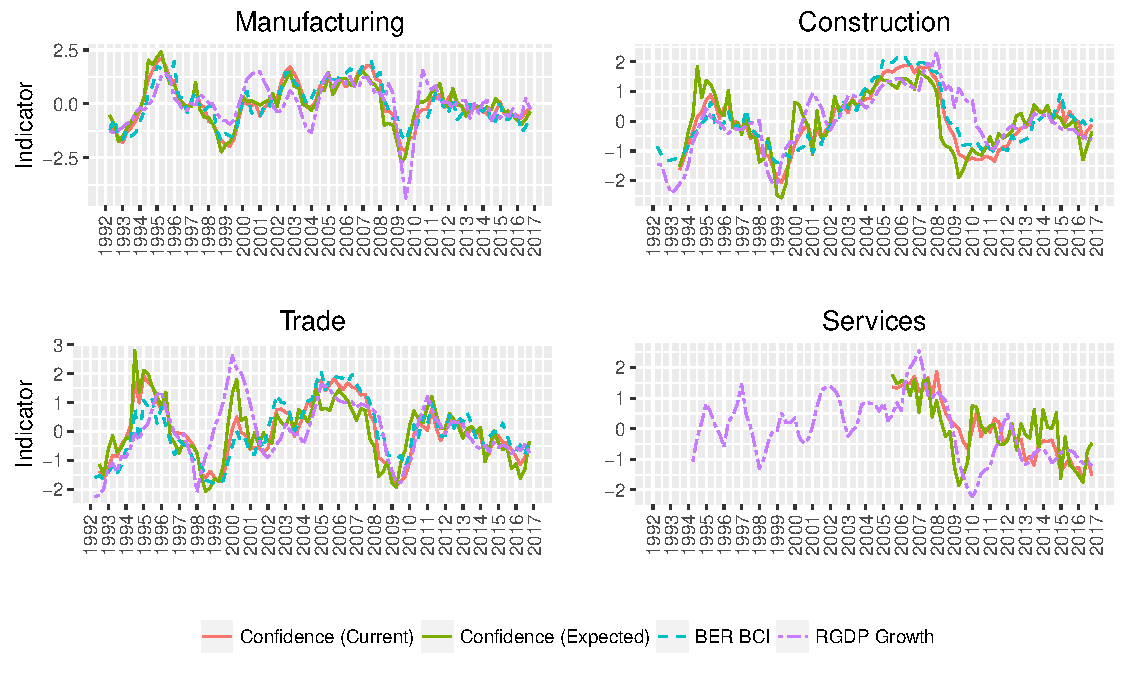
\includegraphics{BCon_5_Journal_files/figure-latex/figure11-1.pdf}
\caption{Sectoral confidence indicators compared to real sectoral GDP
growth}
\end{figure}

The indicators appear to capture cyclical movements in the sectors. In
general, they display an increase in the early 1990s until just after
the first Democratic Elections in 1994Q2. They show a sustained decrease
from 1995 into the recession of 1997-1998, associated with the East
Asian and Russian crises. After troughs around the start of 1999, the
indicators increase up to the global financial crisis at the end of
2007. During this extended upswing phase, the manufacturing and trade
sectors reflect the two ambiguous periods in 2001 and 2003, when
contractions in the SARB leading and coincident indicators obliged an
evaluation of possible reference turning points (Venter, 2005). The
construction sector exhibited a particularly strong and sustained
increase in confidence during this upswing phase, possibly due to the
construction projects associated with hosting the FIFA World Cup in
2010.

The global financial crisis was followed by a large decline in the
indicators for all of the sectors, which continued into the subsequent
Great Recession. There was a relatively quick recovery in confidence in
the manufacturing and trade sectors. Confidence in the construction
sector showed a more gradual recovery, especially in confidence on
current conditions. In the services sector, confidence on current
conditions showed a slight recovery and then continued to decline,
whereas confidence on expected conditions was quite erratic. The
indicators for the other sectors exhibit a gradual decrease from around
2012, continuing into the downswing phase at the end of the sample
period.

Table 3 reports the contemporaneous correlations of the sectoral
indicators and their respective sectoral real GDP growth rates. All the
indicators are highly positively correlated with real sectoral GDP
growth rates. For the most part, the current conditions confidence
indicators exhibit the highest correlation with the reference series. In
this sense, they are an improvement on existing confidence indicators.
The exception is the construction sector, where the BER Building BCI has
the highest correlation. This is peculiar, as the BER Building BCI
includes only building contractors.

\begin{table}[ht]
\centering
\caption{Correlations between sectoral confidence and real sectoral GDP growth} 
\scalebox{0.8}{
\begin{tabular}{|r|lll|lll|}
  \hline
 &   & Manufacturing &   &   & Construction &   \\ 
  \hline
  & Confidence (Cur) & Confidence (Exp) & BER BCI & Confidence (Cur) & Confidence (Exp) & BER BCI \\ \hline
  Confidence (Exp) &  0.94*** &  &  &  0.89*** &  &  \\ 
  BER BCI &  0.92*** &  0.85*** &  &  0.94*** &  0.75*** &  \\ 
  RGDP Growth &  0.68*** &  0.68*** &  0.61*** &  0.74*** &  0.56*** &  0.76*** \\    \hline
  \hline
 &   & Trade &   &   & Services &   \\ 
  \hline
  & Confidence (Cur) & Confidence (Exp) & BER BCI & Confidence (Cur) & Confidence (Exp) & BER BCI \\ \hline
  Confidence (Exp) &  0.87*** &  &  &  0.76*** &  &  \\ 
  BER BCI &  0.90*** &  0.72*** &  &  &  &  \\ 
  RGDP Growth &  0.61*** &  0.59*** &  0.56*** &  0.76*** &  0.57*** &  \\ 
   \hline
\end{tabular}}
\end{table}

Figure 2 illustrates the new aggregate confidence indicators, the BER
and SACCI BCIs, as well as real GDP growth. The indicators appear to be
strongly pro-cyclical, and follow real GDP growth closely. The shaded
areas denote the recessionary periods according to the official turning
points of the SARB. The indicators appear to match the different phases
of the business cycle relatively well, as is discussed in more detail
below.

\begin{figure}
\centering
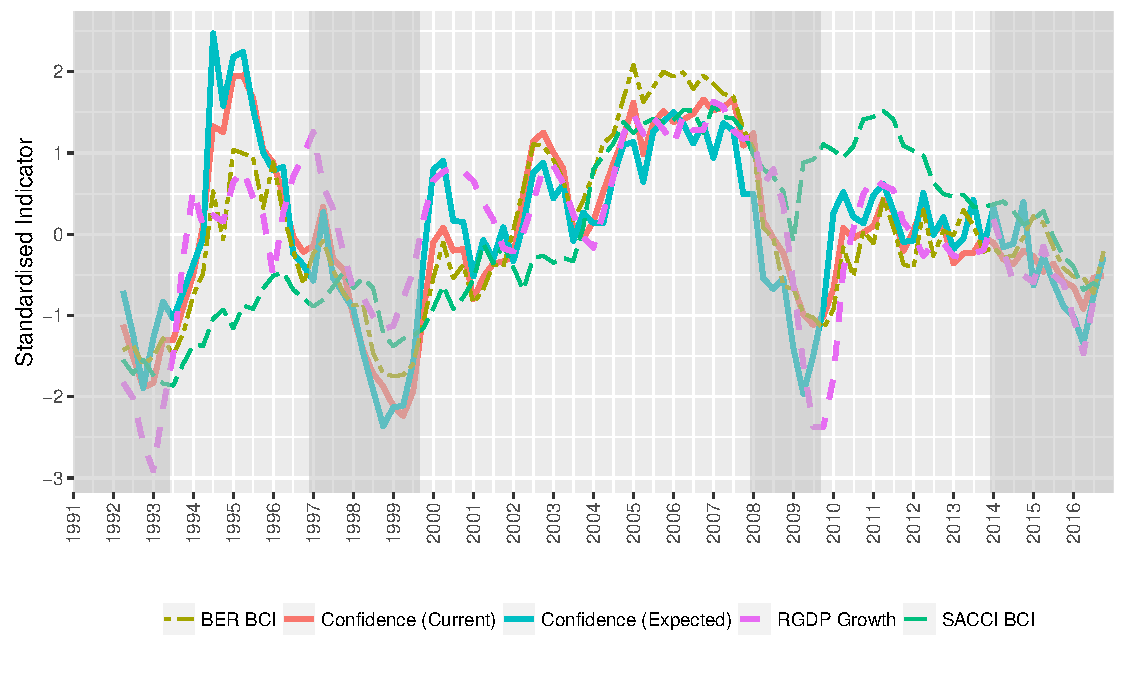
\includegraphics{BCon_5_Journal_files/figure-latex/figure2-1.pdf}
\caption{Aggregate confidence indicators compared to real GDP growth}
\end{figure}

The indicators exhibit an increase following the recession of the early
1990s, with peaks around 1995. There is a prolonged decrease into the
recession of 1997-1998, and a strong recovery just before the official
trough in 1999. Both ambiguous periods are reflected in moderate
decreases in the indicators in 2001 and 2003. Both indicators exhibit a
significant decrease following the global financial crisis in 2007, and
a relatively mild recovery just before the official trough in 2009. The
indicators are relatively flat during the last upswing phase (2010-2013)
and decrease gradually during the downswing phase at the end of the
sample period. The survey-based confidence indicators therefore appear
to be plausible and potentially useful indicators of business confidence
in South Africa.

Table 4 reports the contemporaneous correlations of the indicators and
real GDP growth. SACCI BCI growth rates are used to remove unit roots
and are calculated as annual quarter-on-quarter growth. All the
indicators exhibit a significant positive correlation with one another
and with real GDP growth. The current conditions confidence indicator
has a marginally higher contemporaneous correlation with real GDP growth
than the BER BCI or SACCI BCI. The correlation between the expected
conditions confidence indicator and real GDP growth in the following
quarter is marginally higher than its correlation with contemporaneous
growth. The results suggest that the indicators are all potentially
useful leading or quasi-leading indicators of real activity.

\begin{table}[ht]
\centering
\caption{Correlations between confidence indicators and real GDP growth} 
\scalebox{0.8}{
\begin{tabular}{|r|llll|}
  \hline
 & Confidence (Current) & Confidence (Expected) & BER BCI & SACCI Growth \\ 
  \hline
Confidence (Current) &  &  &  &  \\ 
  Confidence (Expected) &  0.92*** &  &  &  \\ 
  BER BCI &  0.93*** &  0.82*** &  &  \\ 
  SACCI BCI Growth &  0.35*** &  0.48*** &  0.30*** &  \\ \hline
  Real GDP Growth &  0.78*** &  0.70*** &  0.75*** &  0.24**  \\ 
   \hline
\end{tabular}}
\end{table}

\subsubsection{Turning points}\label{turning-points}

An accurate leading indicator should show general conformity to economic
activity (i.e.~a high correlation), as well as a consistent matching of
turning points with the reference cycle. Although there are too few
cycles over the sample period to analyse cyclical turning points in full
detail, it is still of interest to assess whether the indicators behave
in a systematic way around cyclical turning points. In other words, do
they systematically lead, coincide with, or lag the peaks and troughs of
the business cycle.

The turning points in the indicators are determined where they breach
the zero threshold, i.e.~they indicate an upswing when they are positive
and a recession when they are negative. The two new indicators and the
BER BCI are standardised, as their means are below zero over the sample
period, and the SACCI BCI enters in growth rates. Censoring rules are
used to ensure that phases and cycles have a minimum duration, similar
to those used in the so-called Bry-Boschan method (Bry and Boschan,
1971). Following the suggestion of Harding and Pagan (2002), who
developed a variant of this method for dealing with quarterly data (the
BBQ method), a censoring rule based on a minimum of two quarters for
each phase and five quarters for a full cycle is applied.

The resulting phases are illustrated in Figure 3, with the recessionary
periods shaded. The top panel of each graph illustrates the turning
points of the confidence indices, while the bottom panel of each graph
shows the official SARB reference turning points. The sample period
includes three upswing phases and four downswing phases. In addition, in
2001 and 2003 the SARB indicators pointed to possible reference turning
points. Although the SARB dating committee decided at the time that
neither of these periods qualified, subsequent data revisions have shown
that in hindsight there could have been official peaks, especially in
2003, if the dating procedure had been followed mechanically (Venter,
2005).

\begin{figure}
\centering
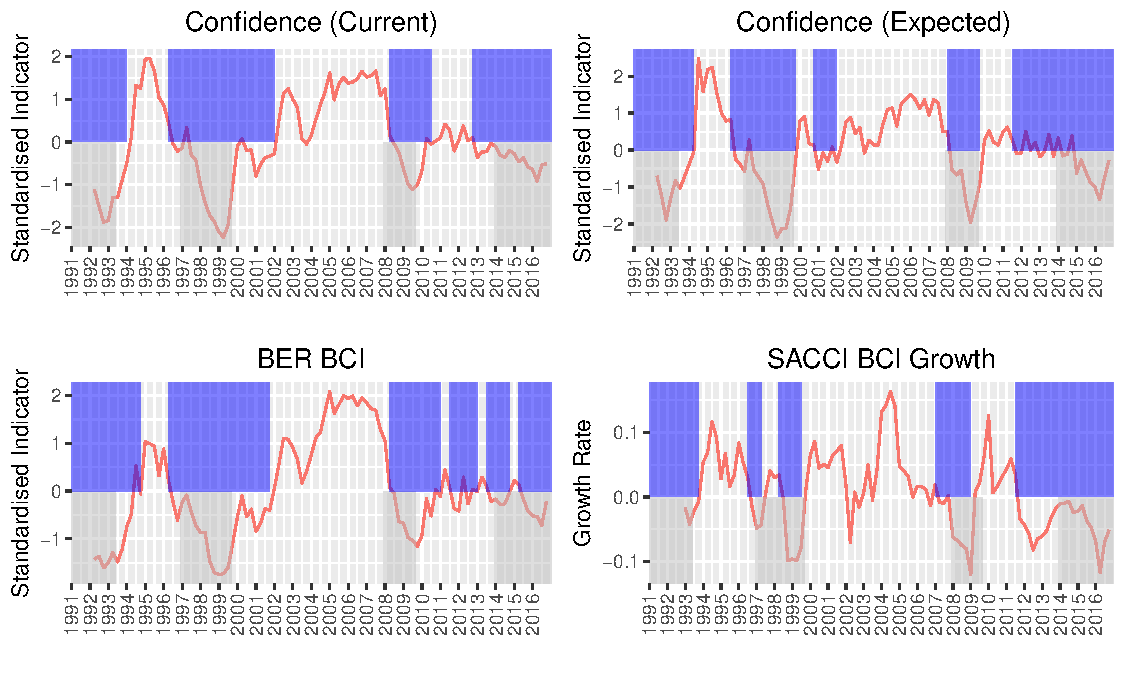
\includegraphics{BCon_5_Journal_files/figure-latex/figure13-1.pdf}
\caption{Confidence indicator turning points compared to the official
SARB turning points}
\end{figure}

The algorithm identifies four recessionary periods in the current
conditions confidence indicator and five in the expected conditions
confidence indicator. These correspond to the official downswing phases,
with the additional downswing phase during the semi-recession in 2001.
The turning points in the BER and SACCI BCIs are similar to those for
the new confidence indicators. There is some ambiguity towards the
latter part of the sample period, as the expected conditions confidence
indicator and the BER BCI hover around the zero threshold. On the whole
the phases identified with the indicators are longer in duration than
the official phases. The indicators mostly exhibit peaks before the
official peak dates, by as many as 10 quarters before the official peak.
The indicators exhibit troughs concurrent with or after the three
official trough dates. The indicators therefore seem to reflect the
official business cycle turning points relatively well.

The comovement between these cycle phases can be measured with the
concordance statistic suggested by Harding and Pagan (2002). The
concordance statistic measures the comovement of two series, by
considering the proportion of time the two series are simultaneously in
the same phase. This entails testing whether \(I=Pr(S_{xt} =S_{yt})\) is
close to 1, where \(S_{xt} = 1\) identifies an expansion in indicator
\(x_t\), and \(S_{yt}=1\) identifies a business cycle upswing phase at
time \(t\). The statistic is calculated as follows:
\(I = 1/T [\sum^T_{t=1} S_{xt} S_{yt} + \sum^T_{t=1} (1-S_{xt}) (1- S_{yt})]\).
Following Harding and Pagan (2006), statistical significance is
calculated with heteroskedasticity and autocorrelation consistent
standard errors.

Table 5 reports the concordance statistics for the phases of the
indicator variables, compared with the official SARB reference turning
points. The indicators all exhibit significant concordance with the
official SARB business cycle. The three survey-based indicators have the
highest concordance statistic with the official SARB cycle when they are
lagged by one or two quarters, but the contemporaneous concordance
statistics are all significant.

\begin{table}[]
\centering
\caption{Concordance statistics with the SARB business cycle}
\scalebox{0.8}{
\begin{tabular}{|r|l|l|l|l|}
\hline
\textbf{}  & \textbf{\begin{tabular}[c]{@{}l@{}}Confidence \\ (Current)\end{tabular}} & \textbf{\begin{tabular}[c]{@{}l@{}}Confidence \\ (Expected)\end{tabular}} & \textbf{BER BCI} & \textbf{\begin{tabular}[c]{@{}l@{}}SACCI \\ BCI Growth\end{tabular}} \\ \hline
lead=3    & 0.60                          & 0.62*                         & 0.47              & 0.72**                 \\
lead=2    & 0.65*                         & 0.67**                        & 0.54              & 0.75***                \\
lead=1    & 0.68**                       & 0.70***                        & 0.59*             & 0.76***                \\
lead/lag=0    & 0.71***                      & 0.73***                       & 0.62**            & 0.75***                \\
lag=1      & 0.72***                      & 0.74***                       & 0.63***           & 0.70***                 \\
lag=2      & 0.73***                      & 0.69***                       & 0.64***           & 0.65***                \\
lag=3      & 0.72***                      & 0.64***                       & 0.63***           & 0.6**                  \\ \hline
\end{tabular}}
\end{table}

The indicators therefore seem to reflect the official business cycle
turning points relatively well, and provided advance warning especially
of the official peaks. The results suggest that the confidence
indicators are potentially useful leading indicators of the business
cycle. However, the false positives and ambiguous periods imply that the
indicators should be used in conjunction with other series when
identifying turning points, as in Laubscher (2014). As more micro-data
from the BER's business tendency surveys become available, the analysis
could be expanded by analysing the cyclical properties of the indicators
in terms of duration, amplitude and steepness.

\subsection{The Impact of Confidence}\label{the-impact-of-confidence-2}

In this section, a simple bivariate VAR is estimated to investigate the
dynamic effects of confidence shocks on the economy. An extended VAR is
then estimated to examine whether the results hold after the inclusion
of additional variables.

\subsubsection{Bivariate VAR Analysis}\label{bivariate-var-analysis}

Impulse response functions (IRFs) can be generated to illustrate the
dynamic impact of a shock to confidence on the system. The shock is an
innovation of one standard deviation to the residual in the equation.
Figure 4 illustrates the IRFs of a bivariate VAR for the confidence
indicator on current conditions and real GDP growth. The left panel
plots the responses of real GDP growth to an orthogonal shock in the
indicator, with 95\% bootstrap confidence intervals.

\begin{figure}
\centering
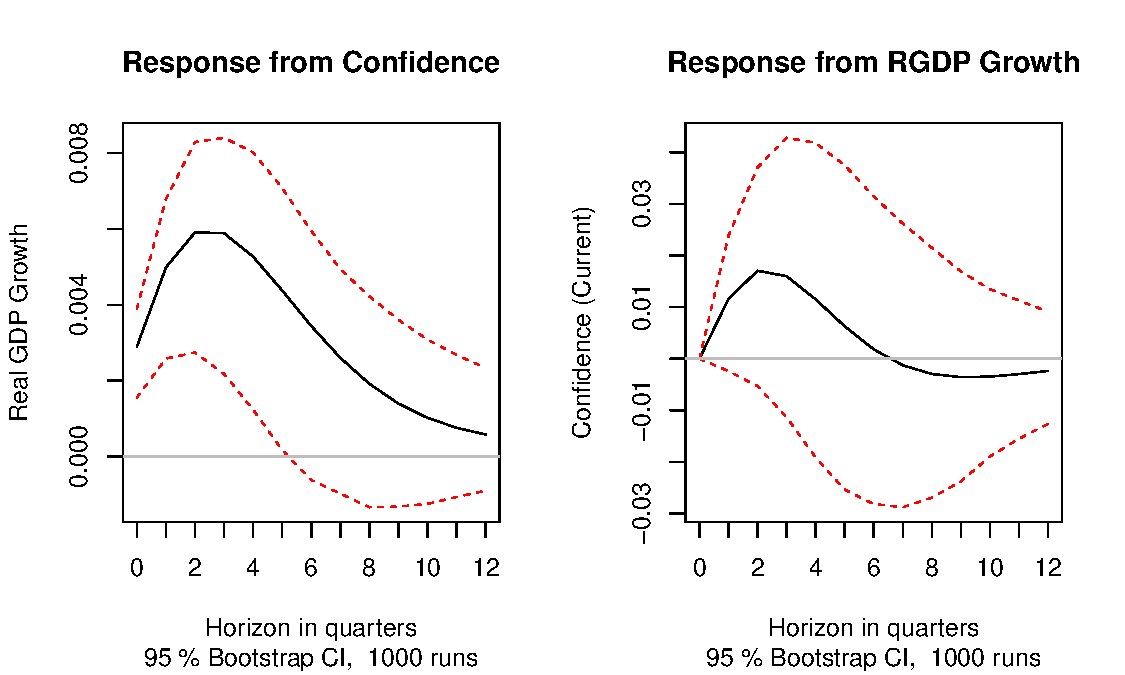
\includegraphics{BCon_5_Journal_files/figure-latex/figure4-1.pdf}
\caption{IRFs of confidence (current conditions) and real GDP growth}
\end{figure}

Following an increase in confidence of one standard deviation, real GDP
growth increases by around 0.3\% on impact, with a peak at two quarters.
The impact on the growth rate is transitory, dying out after
approximately seven quarters. This is equivalent to a permanent increase
in the level of output, which confirms the findings in the literature
(e.g. Barsky and Sims (2012)). The right panel plots the response of
confidence to an orthogonal shock in real GDP growth. Following an
increase in real GDP growth, there is an insignificant increase in
confidence of around 2\% after two quarters. The results are similar for
alternative orderings.

The importance of innovations can also be examined with variance
decompositions. The forecast error variance decomposition (FEVD) shows
the proportion of the movements in a sequence due to its own shocks and
shocks to the other variable. Figure 5 illustrates the FEVDs for the
current conditions confidence indicator and real GDP growth. Up to
around half (46\%) of the movements in real GDP growth are explained by
the confidence indicator over the longer term, while real GDP explains
up to 2\% of the variance in the confidence indicator.

\begin{figure}
\centering
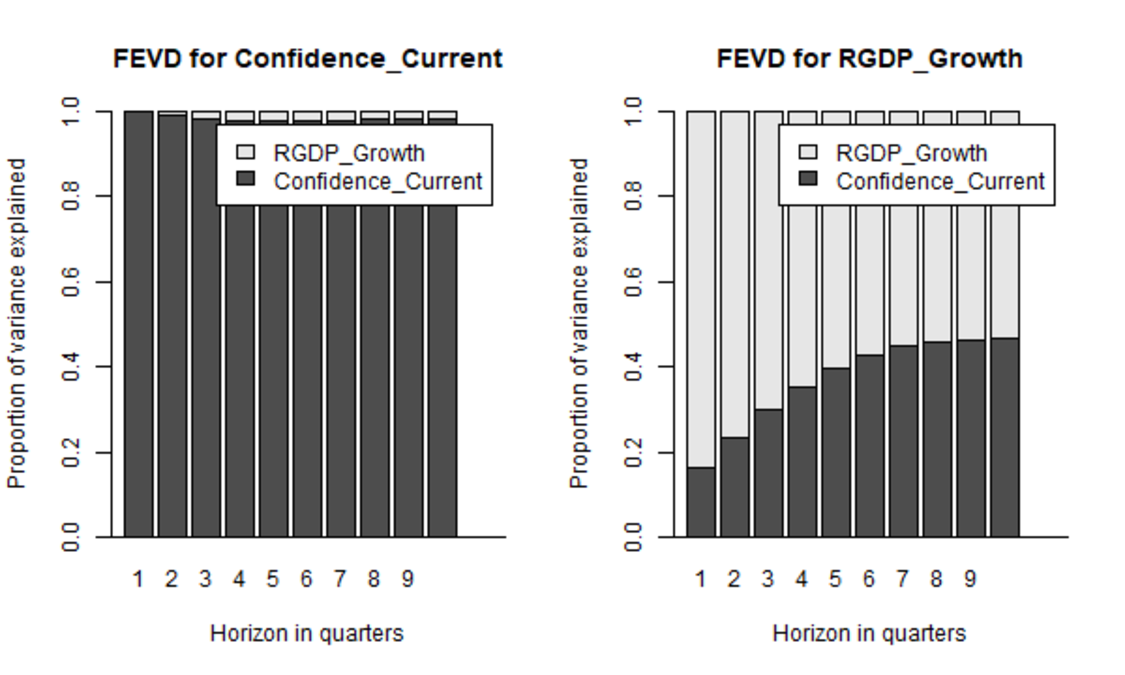
\includegraphics{BCon_5_Journal_files/figure-latex/figure5-1.pdf}
\caption{FEVDs of confidence (current conditions) and real GDP growth}
\end{figure}

The results are very similar when using the expected conditions
confidence indicator and the BER BCI, whereas the SACCI growth rate
exhibits a smaller significant relationship with real GDP growth after
two quarters. The results for the sectoral indicators are also similar
to the aggregate results, with the exception of the construction sector,
where the impact of a shock to confidence on GDP growth does not die out
within the forecast horizon of 12 quarters.

\subsubsection{Expanded VAR}\label{expanded-var}

Though instructive, the results from a bivariate system are prone to
misspecification (Girardi and Reuter, 2017). A larger VAR system is
estimated to test the robustness of the relationships. The extended VAR
includes the variables suggested by Redl (2015) for South Africa:
confidence, the JSE All Share Index, the yield spread (i.e.~the
Government Bond Yield minus the three-month T-Bill rate), an employment
index, and growth in real GDP, industrial production, and investment.
These variables are typically included in the literature (e.g. Leduc and
Liu (2016), Bachmann, Elstner and Sims (2013), and Baker, Bloom and
Davis (2016)).

The confidence indicator is ordered first, the financial variables next,
and the real variables last. The financial variables are expected to
move faster than the real variables (Redl, 2015). An alternative
ordering of placing the confidence indicator last provides qualitatively
similar results. As was the case with the previous VAR, the variables
enter as real annual quarter-on-quarter growth rates, except for
confidence and the yield spread.

The IRFs for the impact of confidence on real GDP, production,
employment and investment growth are illustrated in Figure 6. In this
larger system, a shock to confidence leads to a significant impulse
responses in all four variables. The larger system provides similar
results to the bivariate VAR in terms of the responses of real GDP
growth. The responses of real employment growth are similar in magnitude
to real GDP growth, while the responses of real production and
investment growth are larger. According to the FEVD (not shown),
confidence explains around 35\%, 25\%, 30\%, and 40\% of the variance in
the growth rates in real GDP, production, employment and investment
respectively.

\begin{figure}
\centering
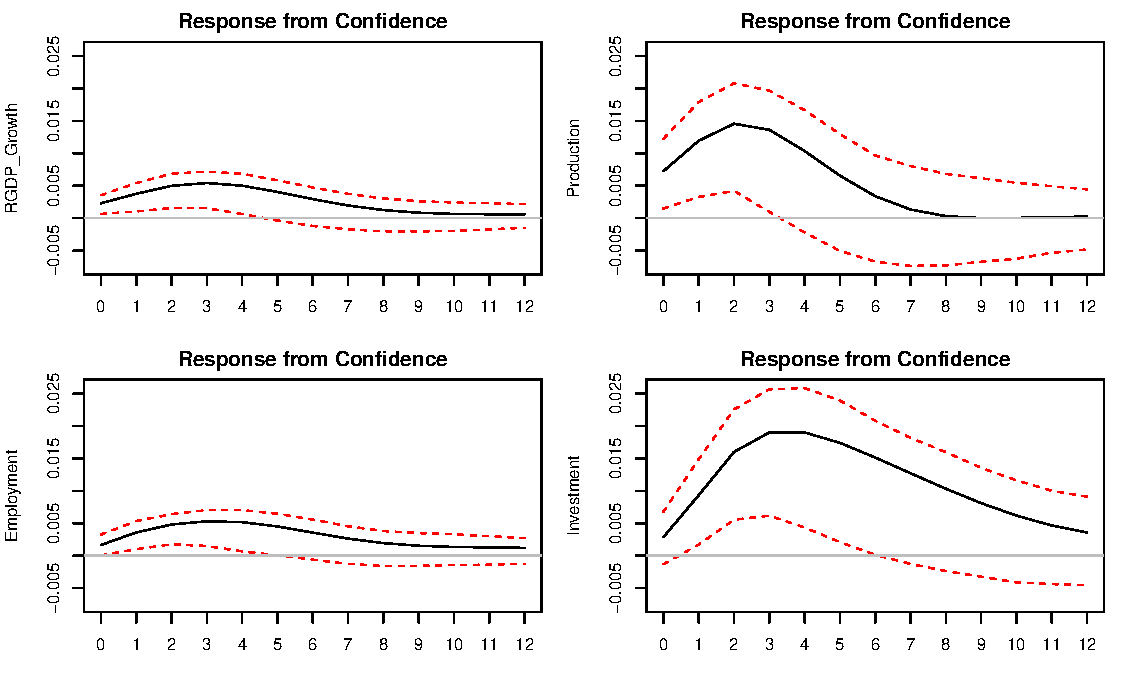
\includegraphics{BCon_5_Journal_files/figure-latex/figure6-1.pdf}
\caption{IRFs of real GDP, production, employment and investment growth
to confidence shocks}
\end{figure}

\section{Conclusion}\label{conclusion}

This chapter has estimated new proxies for business confidence in South
Africa, using micro-data from the BER business tendency surveys, with
the aim of improving on the existing measures. Two sets of composite
confidence indicators were calculated as the weighted cross-sectional
mean of responses to questions on current and expected future business
conditions. The composite current conditions confidence indicator
appeared to be an improvement on existing confidence indicators in that
it exhibited a higher correlation with GDP growth and a higher
concordance statistic with the official SARB business cycle.

The relationship between the business confidence indicators and real
economic activity in South Africa was further examined. The aim was to
study whether there was a significant positive relationship between the
indicators and real GDP growth, the timing of this relationship, and
whether it remained significant after taking other economic variables
into account.

Overall, the results provided evidence at least of significant
comovement between the sectoral and aggregate confidence indicators and
real economic activity. The indicators had a positive and significant
impact on real GDP growth in the VAR models. Shocks to the indicators
accounted for a sizeable fraction of variation in economic activity.
This was the case even after controlling for other economic variables in
a larger VAR system. This implies that the confidence indicators contain
useful predictive content for current and future economic developments.
The indicators may therefore be useful for monitoring developments in
real time and for forecasting future economic activity.

\section*{References}\label{references}
\addcontentsline{toc}{section}{References}

\hypertarget{refs}{}
\hypertarget{ref-Acemoglu1994}{}
Acemoglu, D. and Scott, A. (1994) `Consumer Confidence and Rational
Expectations: Are Agents' Beliefs Consistent with the Theory?',
\emph{The Economic Journal}, 104(January), pp. 1--19.

\hypertarget{ref-Akerlof2015}{}
Akerlof, G. and Shiller, R. J. (2015) \emph{Animal Spirits: How Human
Psychology Drives the Economy, and Why It Matters for Global
Capitalism}. Princeton University Press.

\hypertarget{ref-Bachmann2013}{}
Bachmann, R., Elstner, S. and Sims, E. R. (2013) `Uncertainty and
Economic Activity: Evidence From Business Survey Data', \emph{American
Economic Journal: Macroeconomics}, 5(2), pp. 217--249.

\hypertarget{ref-Baker2016}{}
Baker, S. R., Bloom, N. and Davis, S. J. (2016) `Measuring Economic
Policy Uncertainty', \emph{The Quarterly Journal of Economics}, 131(4),
pp. 1593--1636. doi:
\href{https://doi.org/10.1093/qje/qjw024.Advance}{10.1093/qje/qjw024.Advance}.

\hypertarget{ref-Barsky2012}{}
Barsky, R. B. and Sims, E. R. (2012) `Information, Animal Spirits, and
the Meaning of Innovations in Consumer Confidence', \emph{American
Economic Review}, 102(4), pp. 1343--1377. doi:
\href{https://doi.org/10.1257/aer.102.4.1343}{10.1257/aer.102.4.1343}.

\hypertarget{ref-Beaudry2004}{}
Beaudry, P. and Portier, F. (2004) `An Exploration into Pigou's Theory
of Cycles', \emph{Journal of Monetary Economics}, 51(6), pp. 1183--1216.
doi:
\href{https://doi.org/10.1016/j.jmoneco.2003.10.003}{10.1016/j.jmoneco.2003.10.003}.

\hypertarget{ref-Bosch2015}{}
Bosch, A. (2015) `Composite Business Cycle Indicators for South Africa',
\emph{South African Reserve Bank}, (24 March 2015).

\hypertarget{ref-Bry1971}{}
Bry, G. and Boschan, C. (1971) `Programmed Selection Of Cyclical Turning
Points', \emph{National Bureau of Economic Research}, I, pp. 7--63.

\hypertarget{ref-Carroll1994}{}
Carroll, C. D., Fuhrer, J. C. and Wilcox, D. W. (1994) `Does Consumer
Sentiment Forecast Household Spending? If So, Why?', \emph{American
Economic Review}, 84(5), pp. 1397--1408.

\hypertarget{ref-Cochrane1994}{}
Cochrane, J. H. (1994) `Shocks', \emph{Carnegie-Rochester Conference
Series on Public Policy}, 41(December 1994), pp. 295--364.

\hypertarget{ref-Driver2004}{}
Driver, C. and Urga, G. (2004) `Transforming Qualitative Survey Data:
Performance Comparisons for the UK', \emph{Oxford Bulletin of Economics
and Statistics}, 66(1), pp. 71--89. doi:
\href{https://doi.org/10.1111/j.1440-1754.2007.01273.x}{10.1111/j.1440-1754.2007.01273.x}.

\hypertarget{ref-ECB2013}{}
European Central Bank (2013) `Confidence Indicators and Economic
Developments', \emph{ECB Monthly Bulletin}, (January), pp. 45--58.

\hypertarget{ref-EC2006}{}
European Commission (2006) \emph{European Economies: The Joint
Harmonised EU Programme of Business and Consumer Surveys}.
Directorate-General for Economic; Financial Affairs (Special Report No.
5).

\hypertarget{ref-Fuhrer1988}{}
Fuhrer, J. C. (1988) `On the Information Content of Consumer Survey
Expectations', \emph{The Review of Economics and Statistics}, pp.
140--144.

\hypertarget{ref-Gayer2014}{}
Gayer, C., Girardi, A. and Reuter, A. (2014) `The Role of Survey Data in
Nowcasting Euro Area GDP Growth', \emph{European Commission Economic
Papers}, 538(December). doi:
\href{https://doi.org/10.2765/71951}{10.2765/71951}.

\hypertarget{ref-Gehlbach2012}{}
Gehlbach, H. and Barge, S. (2012) `Anchoring and Adjusting in
Questionnaire Responses', \emph{Basic and Applied Social Psychology},
34(5 (September)), pp. 417--433. doi:
\href{https://doi.org/10.1080/01973533.2012.711691}{10.1080/01973533.2012.711691}.

\hypertarget{ref-Giannone2008}{}
Giannone, D., Reichlin, L. and Small, D. (2008) `Nowcasting: The
Real-Time Informational Content of Macroeconomic Data', \emph{Journal of
Monetary Economics}, 55(June), pp. 665--676. doi:
\href{https://doi.org/10.1016/j.jmoneco.2008.05.010}{10.1016/j.jmoneco.2008.05.010}.

\hypertarget{ref-Girardi2017}{}
Girardi, A. and Reuter, A. (2017) `New Uncertainty Measures for the Euro
Area Using Survey Data', \emph{Oxford Economic Papers}, 69(1), pp.
278--300. doi:
\href{https://doi.org/10.1093/oep/gpw058}{10.1093/oep/gpw058}.

\hypertarget{ref-Harding2002}{}
Harding, D. and Pagan, A. (2002) `Dissecting the Cycle: A Methodological
Investigation', \emph{Journal of Monetary Economics}, 49(2), pp.
365--381. doi:
\href{https://doi.org/10.1016/S0304-3932(01)00108-8}{10.1016/S0304-3932(01)00108-8}.

\hypertarget{ref-Harding2006}{}
Harding, D. and Pagan, A. (2006) `Synchronization of Cycles',
\emph{Journal of Econometrics}, 132, pp. 59--79. doi:
\href{https://doi.org/10.1016/j.jeconom.2005.01.023}{10.1016/j.jeconom.2005.01.023}.

\hypertarget{ref-IMF2017}{}
International Monetary Fund (2017) `World Economic Outlook Update',
\emph{IMF Publications}, July 23.

\hypertarget{ref-Kabundi2004}{}
Kabundi, A. (2004) `Estimation of Economic Growth in France Using
Business Survey Data', \emph{IMF Working Paper}, WP/04/69.

\hypertarget{ref-Kabundi2016}{}
Kabundi, A., Nel, E. and Ruch, F. (2016) `Nowcasting Real GDP Growth in
South Africa', \emph{ERSA Working Paper}, 581.

\hypertarget{ref-Kershoff2000}{}
Kershoff, G. (2000) `Measuring Business and Consumer Confidence in South
Africa', \emph{Bureau for Economic Research}, (December).

\hypertarget{ref-Kershoff2002}{}
Kershoff, G. (2002) `An Analysis of The BER's Trade and Building Survey
Panels', \emph{Journal for Studies in Economics and Econometrics},
26(1), pp. 1--17.

\hypertarget{ref-Kershoff2015}{}
Kershoff, G. (2015) `South Africa: The BER's Business Tendency Surveys',
\emph{Bureau for Economic Research}, pp. 1--19.

\hypertarget{ref-Keynes1936}{}
Keynes, J. M. (1936) \emph{General Theory of Employment, Interest and
Money}. London: Macmillan. doi:
\href{https://doi.org/10.2307/2143949}{10.2307/2143949}.

\hypertarget{ref-Kilic2016}{}
Kilic, E. and Cankaya, S. (2016) `Consumer Confidence and Economic
Activity: A Factor Augmented VAR Approach', \emph{Applied Economics},
48(32), pp. 3062--3080. doi:
\href{https://doi.org/10.1080/00036846.2015.1133902}{10.1080/00036846.2015.1133902}.

\hypertarget{ref-Laubscher2014}{}
Laubscher, P. (2014) `A New Recession-Dating Algorithm for South
Africa', \emph{Stellenbosch Economic Working Papers}, 06/14.

\hypertarget{ref-Leduc2016}{}
Leduc, S. and Liu, Z. (2016) `Uncertainty Shocks are Aggregate Demand
Shocks', \emph{Journal of Monetary Economics}. Elsevier, 82, pp. 20--35.
doi:
\href{https://doi.org/10.1016/j.jmoneco.2016.07.002}{10.1016/j.jmoneco.2016.07.002}.

\hypertarget{ref-Leduc2013}{}
Leduc, S. and Sill, K. (2013) `Expectations and Economic Fluctuations:
An Analysis Using Survey Data', \emph{Review of Economics and
Statistics}, 95(October), pp. 1352--1367.

\hypertarget{ref-Ludvigson2004}{}
Ludvigson, S. C. (2004) `Consumer Confidence and Consumer Spending',
\emph{Journal of Economic Perspectives}, 18(2), pp. 29--50.

\hypertarget{ref-Matheson2010}{}
Matheson, T. D. (2010) `An Analysis of the Informational Content of New
Zealand Data Releases: The Importance of Business Opinion Surveys',
\emph{Economic Modelling}. Elsevier B.V., 27(1), pp. 304--314. doi:
\href{https://doi.org/10.1016/j.econmod.2009.09.010}{10.1016/j.econmod.2009.09.010}.

\hypertarget{ref-Mendicino2013}{}
Mendicino, C. and Punzi, M. T. (2013) `Confidence and Economic Activity:
The Case of Portugal', \emph{Banco de Portugal}, (Winter), pp. 39--49.

\hypertarget{ref-Nardo2003}{}
Nardo, M. (2003) `The Quantification of Qualitative Survey Data: A
Critical Assessment', \emph{Journal of Economic Surveys}, 17(5), pp.
645--668.

\hypertarget{ref-OECD2003}{}
Organisation for Economic Co-operation and Development (2003)
\emph{Business Tendency Surveys: A Handbook}. Edited by E. Giovannini
and E. Burgeat. Paris, France: OECD Publications.

\hypertarget{ref-Parigi2004}{}
Parigi, G. and Golinelli, R. (2004) `Consumer Sentiment and Economic
Activity', \emph{Journal of Business Cycle Measurement and Analysis},
2004(2), pp. 147--170. doi:
\href{https://doi.org/10.1787/jbcma-v2004-art10-en}{10.1787/jbcma-v2004-art10-en}.

\hypertarget{ref-Pellissier2002}{}
Pellissier, M. (2002) `Business Confidence and the South African
Business Cycle', \emph{Journal for Studies in Economics and
Econometrics}, 26(2), pp. 51--67.

\hypertarget{ref-Redl2015}{}
Redl, C. (2015) `Macroeconomic Uncertainty in South Africa', \emph{ERSA
Working Paper}, 509.

\hypertarget{ref-SACCI2011}{}
SACCI (2011) `Updated and Revised SACCI Business Confidence Index',
\emph{South African Chamber of Commerce and Industry}.

\hypertarget{ref-Santero1996}{}
Santero, T. and Westerlund, N. (1996) `Confidence Indicators and Their
Relationship to Changes in Economic Activity', \emph{OECD Economics
Department Working Papers}, 170. doi:
\href{https://doi.org/10.1787/537052766455}{10.1787/537052766455}.

\hypertarget{ref-Taylor2007}{}
Taylor, K. and McNabb, R. (2007) `Business Cycles and the Role of
Confidence: Evidence for Europe', \emph{Oxford Bulletin of Economics and
Statistics}, 69(2), pp. 185--208. doi:
\href{https://doi.org/10.1111/j.1468-0084.2007.00472.x}{10.1111/j.1468-0084.2007.00472.x}.

\hypertarget{ref-Tversky1974}{}
Tversky, A. and Kahneman, D. (1974) `Judgment under Uncertainty:
Heuristics and Biases', \emph{Science}, 185(4157), pp. 1124--1131.

\hypertarget{ref-UN2015}{}
United Nations (2015) \emph{Handbook on Economic Tendency Surveys}. New
York: United Nations Publications.

\hypertarget{ref-VanAarle2012}{}
Van Aarle, B. and Kappler, M. (2012) `Economic Sentiment Shocks and
Fluctuations in Economic Activity in the Euro Area and the USA',
\emph{Intereconomics}, 47(1), pp. 44--51. doi:
\href{https://doi.org/10.1007/s10272-012-0405-z}{10.1007/s10272-012-0405-z}.

\hypertarget{ref-Venter2005a}{}
Venter, J. C. (2005) `Reference Turning Points in the South African
Business Cycle: Recent Developments', \emph{SARB Quarterly Bulletin},
(September), pp. 61--70.


\end{document}
